\documentclass{beamer}

\usetheme{Montpellier}

\usepackage{graphicx}
\usepackage{amsmath}

\setbeamertemplate{headline}{}


\title{Review of methods}
\author{Andrea Bonifacio}

\begin{document}
\beamertemplatenavigationsymbolsempty
\begin{frame}
\titlepage
\end{frame}

\begin{frame}
\frametitle{Spatial super-resolution}
\begin{columns}
\column{0.4\textwidth}

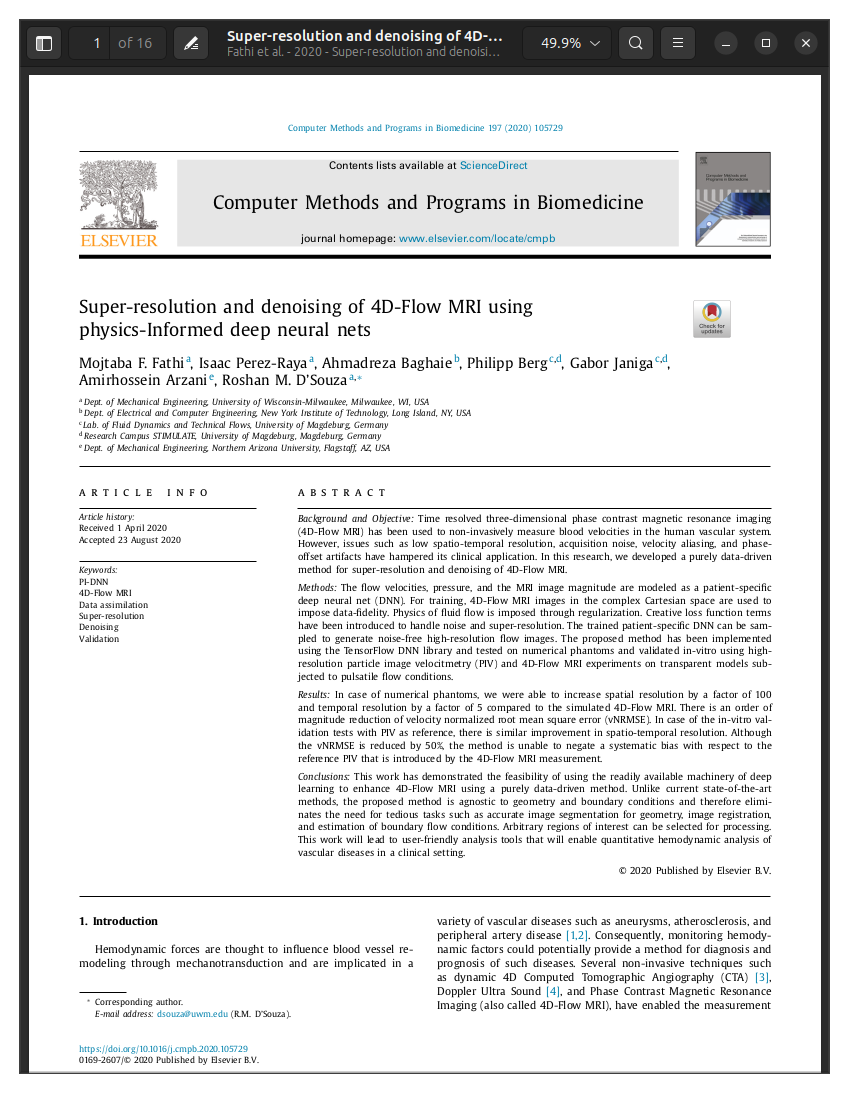
\includegraphics[scale=0.13]{figures/PINN_SuperResolution.png}
\column{0.6\textwidth}
\begin{itemize}
    \item Needs only coarse simulation data
    \item Physics must be implemented
    \item Grid-dependent
    \item Spatial deformation only
    \item Not clear the treatment of boundaries
\end{itemize}
\end{columns}
\end{frame}

\begin{frame}
    \frametitle{Spatial super-resolution}
\begin{columns}
\column{0.5\textwidth}
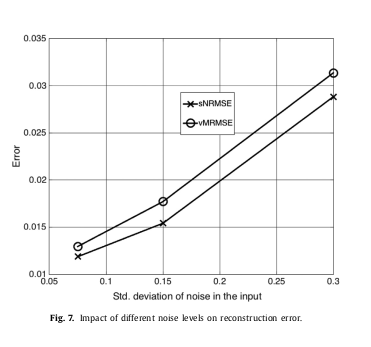
\includegraphics[scale=0.4]{figures/PINN_error.png}
\column{0.5\textwidth}
\begin{itemize}
    \item Good reconstruction error with low level of noise
\end{itemize}
\end{columns}
\end{frame}

\begin{frame}
    \frametitle{Multiscale MeshGraphNet}
\begin{columns}
\column{0.4\textwidth}
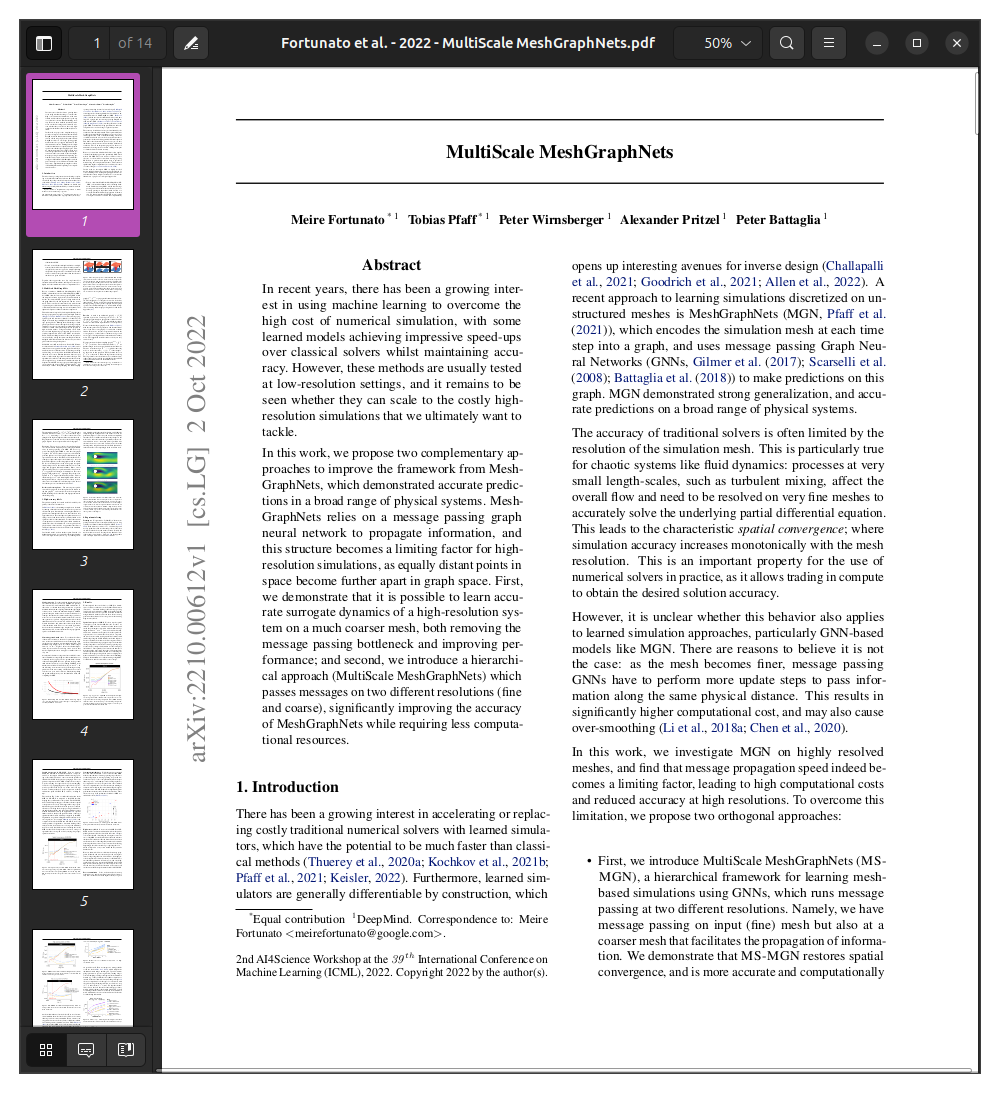
\includegraphics[scale=0.13]{figures/MultiscaleMGN.png}
\column{0.6\textwidth}
\begin{itemize}
    \item Both coarse and fine data needed
    \item No physics information
    \item Grid-independent
    \item Spatial deformation and temporal evolution
    \item Black-box method
\end{itemize}
\end{columns}
\end{frame}

\begin{frame}
    \frametitle{Multiscale MeshGraphNet}
\begin{columns}
\column{0.5\textwidth}
\includegraphics[scale=0.2]{figures/MGN_error.png}
\column{0.5\textwidth}
\begin{itemize}
    \item Good reconstruction error at various mesh sizes
    \item Higher accuracy than classical solver at low mesh sizes
\end{itemize}
\end{columns}
\end{frame}

\begin{frame}
    \frametitle{Transformer}
\begin{columns}
\column{0.4\textwidth}
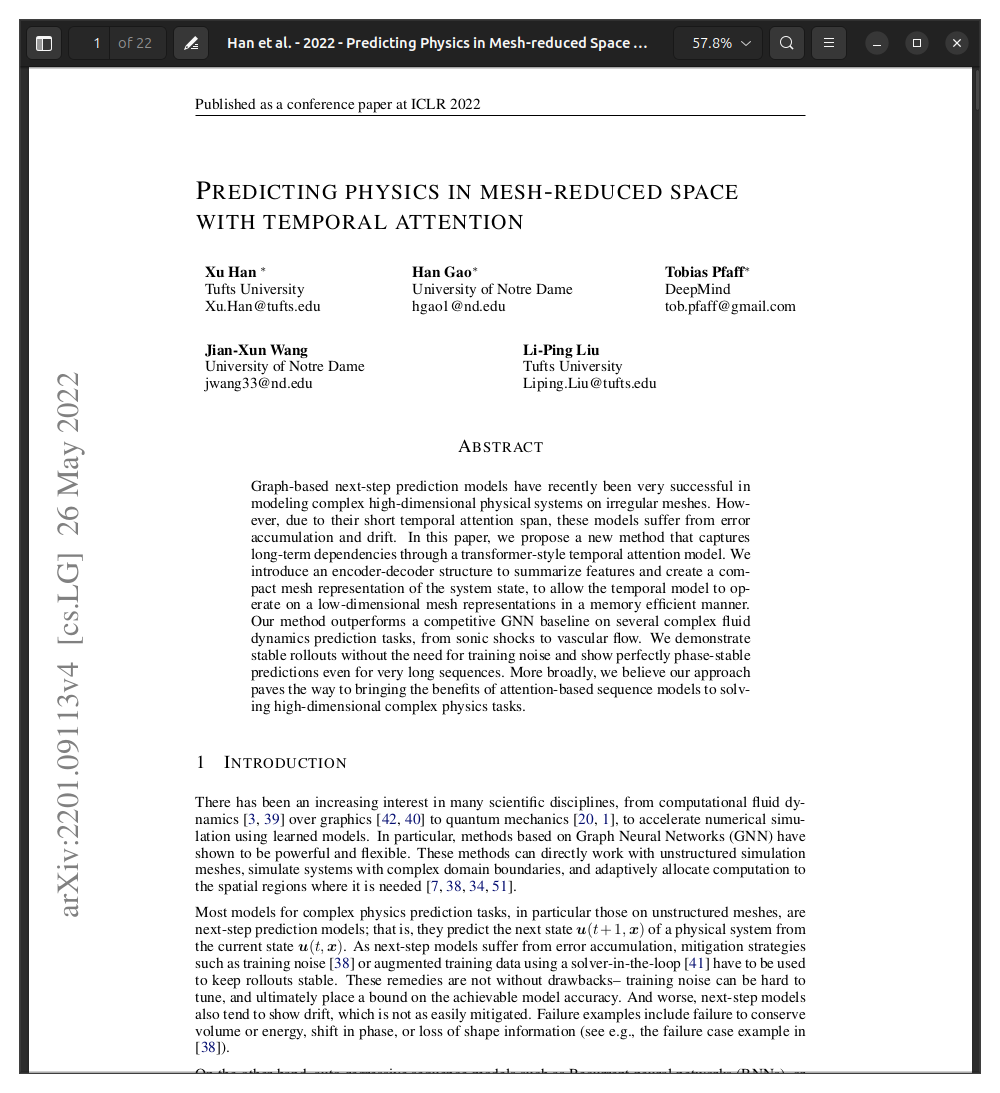
\includegraphics[scale=0.12]{figures/Transformer.png}
\column{0.6\textwidth}
\begin{itemize}
    \item Only fine data needed
    \item No physics information
    \item Grid-independent
    \item Spatial deformation and temporal evolution
    \item Black-box method
\end{itemize}
\end{columns}
\end{frame}

\begin{frame}
    \frametitle{Transformer}
\begin{columns}
\column{0.5\textwidth}
\includegraphics[scale=0.2]{figures/Transformer_error.png}
\column{0.5\textwidth}
\begin{itemize}
    \item Little error accumulation
    \item Much better than MGN
\end{itemize}
\end{columns}
\end{frame}

\begin{frame}
    \frametitle{Physics-informed Graph Networks}
\begin{columns}
\column{0.4\textwidth}
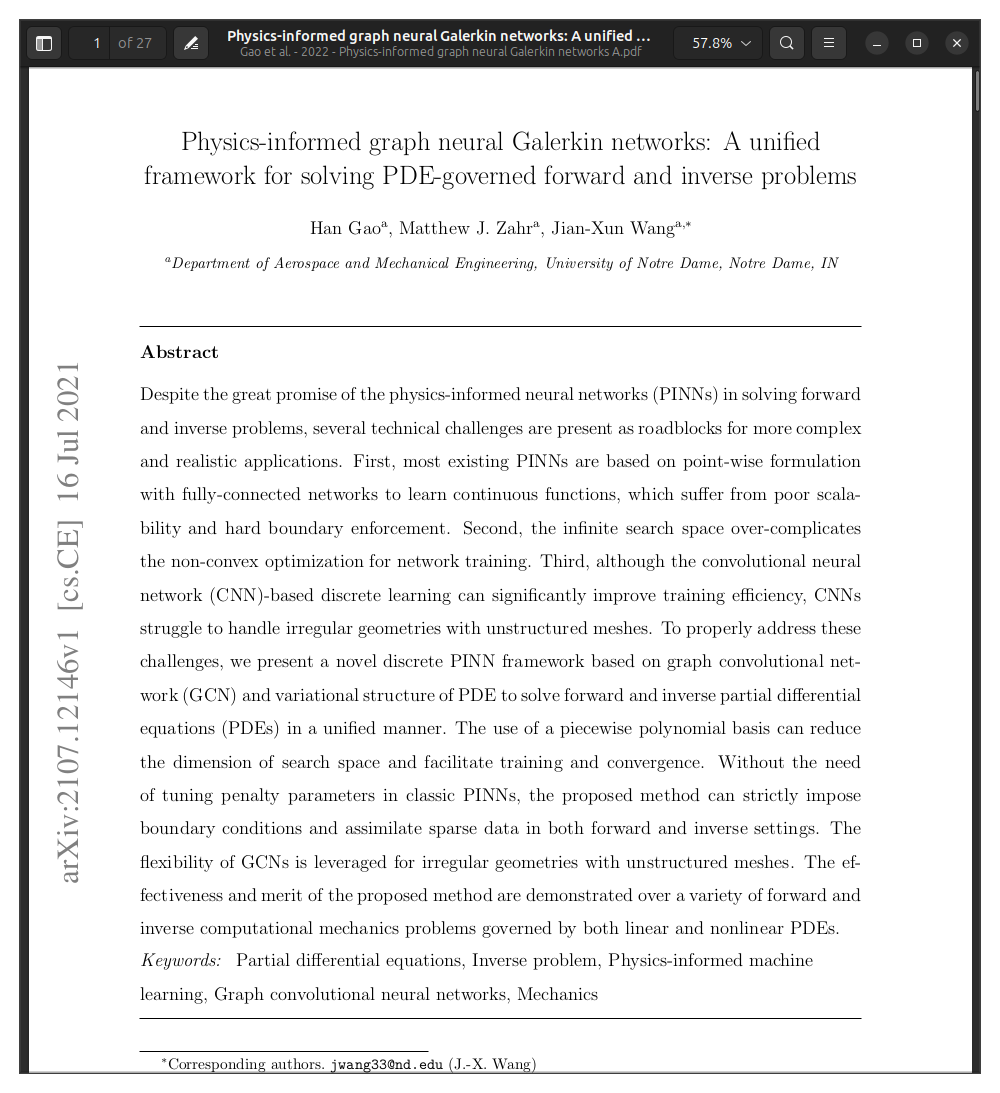
\includegraphics[scale=0.12]{figures/PIGNN.png}
\column{0.6\textwidth}
\begin{itemize}
    \item Point-wise training
    \item Physics must be implemented
    \item Irregular meshes
    \item Spatial deformation
\end{itemize}
\end{columns}
\end{frame}

\begin{frame}
    \frametitle{Physics-informed Graph Networks}
\begin{columns}
\column{0.5\textwidth}
\includegraphics[scale=0.2]{figures/PIGNN_error.png}
\column{0.5\textwidth}
\begin{itemize}
    \item Little error on simple test cases
    \item Tested on deformation problems
\end{itemize}
\end{columns}
\end{frame}

\begin{frame}
    \frametitle{MeshFreeFlowNet}
\begin{columns}
\column{0.4\textwidth}
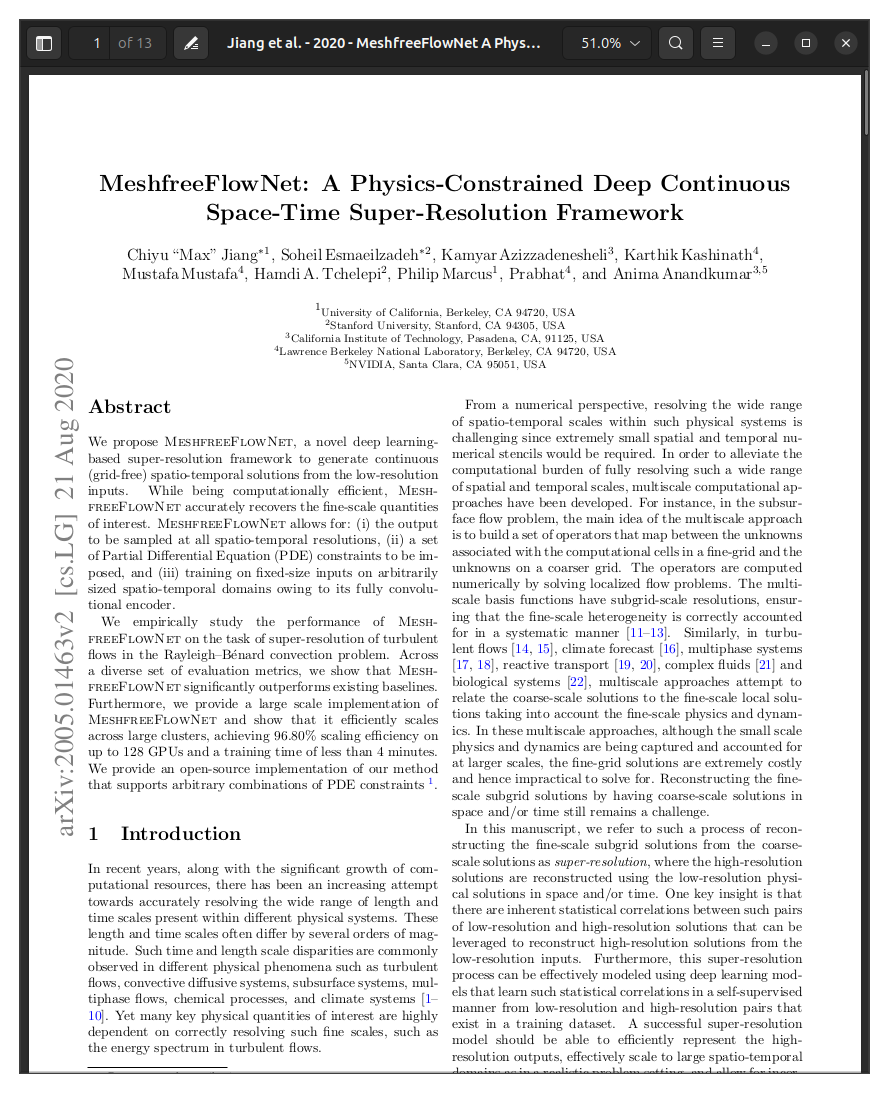
\includegraphics[scale=0.12]{figures/MeshFreeFlowNet.png}
\column{0.6\textwidth}
\begin{itemize}
    \item Both coarse and fine data needed
    \item No physics information
    \item U-net as deep learning model
    \item Spatial deformation and temporal evolution
    \item Black-box method
\end{itemize}
\end{columns}
\end{frame}

\begin{frame}
    \frametitle{MeshFreeFlowNet}
\begin{columns}
\column{0.5\textwidth}
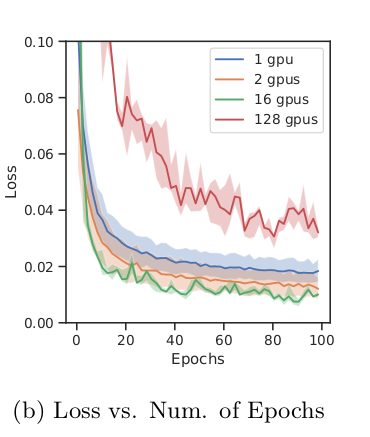
\includegraphics[scale=0.3]{figures/MeshFreeFlowNet_Error.png}
\column{0.5\textwidth}
\begin{itemize}
    \item No clear information about the error, but not a good loss
    \item Tested on fluid dynamics
    \item Familiar method with U-Net
\end{itemize}
\end{columns}
\end{frame}

\begin{frame}
    \frametitle{Why not CNN?}
\begin{columns}
\column{0.4\textwidth}
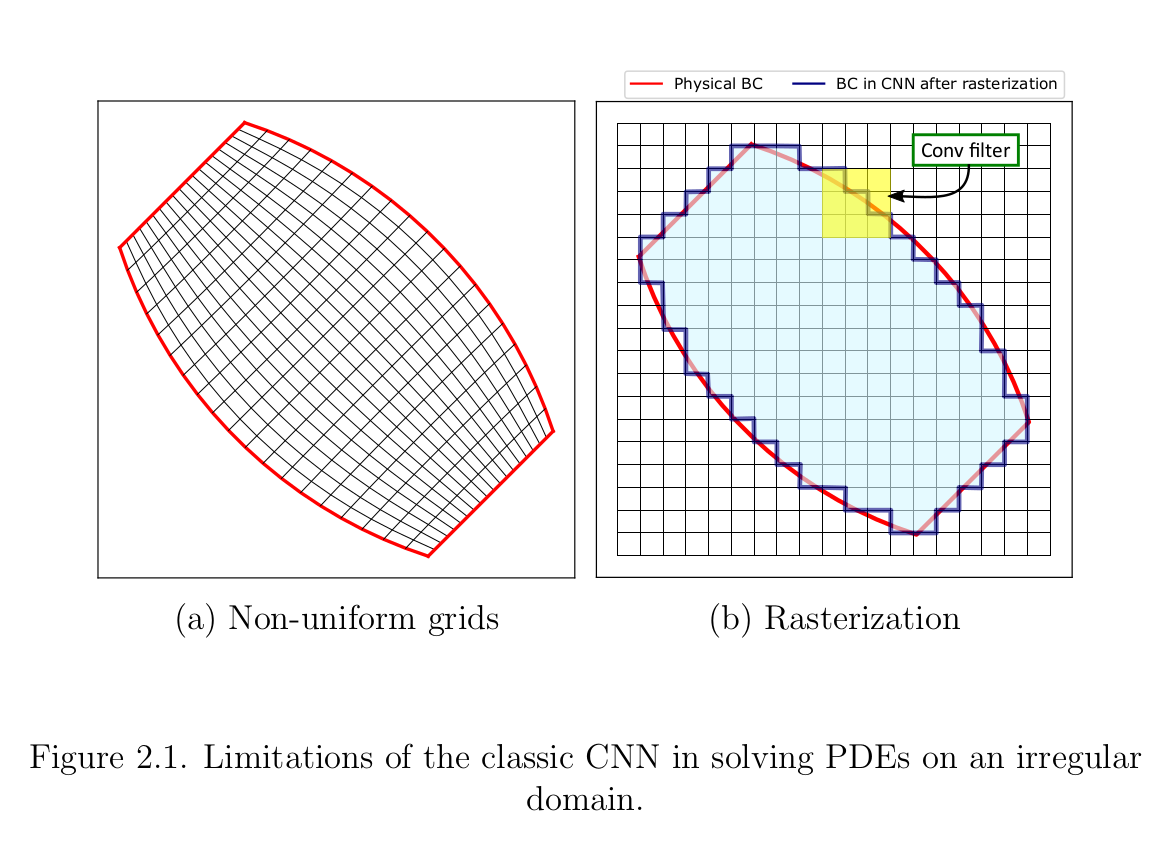
\includegraphics[scale=0.1]{figures/CNN_Limitations.png}

\column{0.6\textwidth}
\begin{itemize}
    \item CNN is not suitable for irregular meshes
    \item Generates problems at boundaries
    \item A lot of solution for fluid dynamics are based on it, but seems impractical for lagrangian problems
\end{itemize}
\end{columns}
\end{frame}

\begin{frame}
    \frametitle{AMG with GNN}
\begin{columns}
\column{0.4\textwidth}
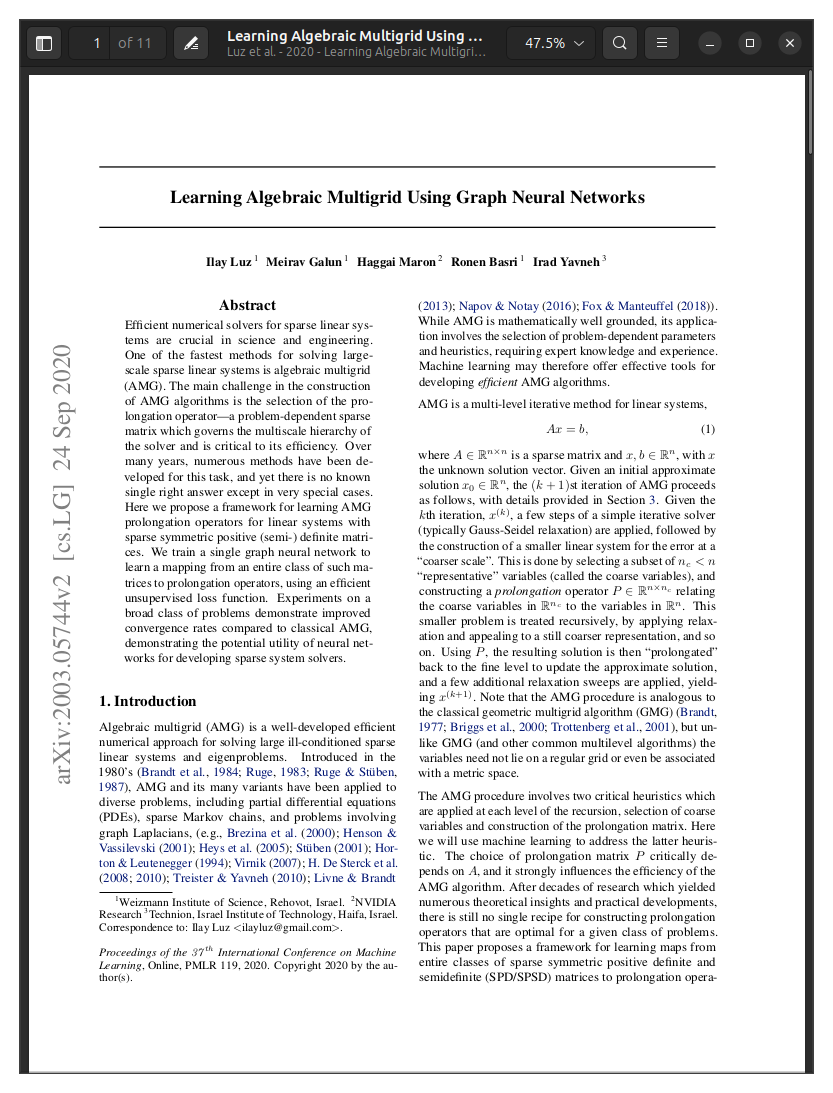
\includegraphics[scale=0.1]{figures/AMG.png}

\column{0.6\textwidth}
\begin{itemize}
    \item Acts directly on the solver
    \item Little to no error accumulation
    \item Probably very difficult to implement
    \item Still in the black box category
\end{itemize}
\end{columns}
\end{frame}

\begin{frame}
    \frametitle{Recap}
\begin{columns}
\column{0.5\textwidth}
\centering \textbf{Spatial deformation}
\begin{itemize}
    \item PINN
    \item PIGNN
    \item AMG GNN
\end{itemize}
\column{0.5\textwidth}
\centering \textbf{Temporal evolution}
\begin{itemize}
    \item MGN
    \item Transformer
    \item MeshFreeFlowNet
\end{itemize}
\end{columns}
\end{frame}
\end{document}